%%%%%%%%%%%%%%%%%%%%%%%%%%%%%%%%%%%%%%%%%%%%%%%%%%%%%%%%%%%%%%%%
%
%  Template for homework of Introduction to Machine Learning.
%
%  Fill in your name, lecture number, lecture date and body
%  of homework as indicated below.
%
%%%%%%%%%%%%%%%%%%%%%%%%%%%%%%%%%%%%%%%%%%%%%%%%%%%%%%%%%%%%%%%%


\documentclass[11pt,letter,notitlepage]{article}
%Mise en page
\usepackage[left=2cm, right=2cm, lines=45, top=0.8in, bottom=0.7in]{geometry}
\usepackage{ctex}
\usepackage{fancyhdr}
\usepackage{fancybox}
\usepackage{graphicx}
\usepackage{pdfpages} 
\usepackage{enumitem}
\usepackage{algorithm}
\usepackage{algorithmic}
\renewcommand{\headrulewidth}{1.5pt}
\renewcommand{\footrulewidth}{1.5pt}
\newcommand\Loadedframemethod{TikZ}
\usepackage[framemethod=\Loadedframemethod]{mdframed}

\usepackage{amssymb,amsmath}
\usepackage{amsthm}
\usepackage{thmtools}
\newtheorem{lemma}{Lemma}

\setlength{\topmargin}{0pt}
\setlength{\textheight}{9in}
\setlength{\headheight}{0pt}

\setlength{\oddsidemargin}{0.25in}
\setlength{\textwidth}{6in}

\usepackage{graphicx} % more modern
\usepackage{subfigure}
\usepackage{threeparttable}

%%%%%%%%%%%%%%%%%%%%%%%%
%%%%%% Define math operator %%%%%
%%%%%%%%%%%%%%%%%%%%%%%%
\DeclareMathOperator*{\argmin}{\bf argmin}
\DeclareMathOperator*{\argmax}{\bf argmax}
\DeclareMathOperator*{\relint}{\bf relint\,}
\DeclareMathOperator*{\dom}{\bf dom\,}
\DeclareMathOperator*{\intp}{\bf int\,}
\DeclareMathOperator*{\tr}{\bf tr\,}
%%%%%%%%%%%%%%%%%%%%%%%


\setlength{\topmargin}{0pt}
\setlength{\textheight}{9in}
\setlength{\headheight}{0pt}

\setlength{\oddsidemargin}{0.25in}
\setlength{\textwidth}{6in}
\pagestyle{fancy}
%%%%%%%%%%%%%%%%%%%%%%%%
%% Define the Exercise environment %%
%%%%%%%%%%%%%%%%%%%%%%%%
\mdtheorem[
topline=false,
rightline=false,
leftline=false,
bottomline=false,
leftmargin=-10,
rightmargin=-10
]{exercise}{\textbf{Exercise}}
%%%%%%%%%%%%%%%%%%%%%%%
%% End of the Exercise environment %%
%%%%%%%%%%%%%%%%%%%%%%%


%%%%%%%%%%%%%%%%%%%%%%%%
%% Define the Problem environment %%
%%%%%%%%%%%%%%%%%%%%%%%%
\mdtheorem[
topline=false,
rightline=false,
leftline=false,
bottomline=false,
leftmargin=-10,
rightmargin=-10
]{problem}{\textbf{Problem}}
%%%%%%%%%%%%%%%%%%%%%%%
%% End of the Exercise environment %%
%%%%%%%%%%%%%%%%%%%%%%%

%%%%%%%%%%%%%%%%%%%%%%%
%% Define the Solution Environment %%
%%%%%%%%%%%%%%%%%%%%%%%
\declaretheoremstyle
[
spaceabove=0pt, 
spacebelow=0pt, 
headfont=\normalfont\bfseries,
notefont=\mdseries, 
notebraces={(}{)}, 
headpunct={:\quad}, 
headindent={},
postheadspace={ }, 
postheadspace=4pt, 
bodyfont=\normalfont, 
qed=$\blacksquare$,
preheadhook={\begin{mdframed}[style=myframedstyle]},
	postfoothook=\end{mdframed},
]{mystyle}

\declaretheorem[style=mystyle,title=Solution,numbered=no]{solution}
\mdfdefinestyle{myframedstyle}{%
	topline=false,
	rightline=false,
	leftline=false,
	bottomline=false,
	skipabove=-6ex,
	leftmargin=-10,
	rightmargin=-10}
%%%%%%%%%%%%%%%%%%%%%%%
%% End of the Solution environment %%
%%%%%%%%%%%%%%%%%%%%%%%

%% Homework info.
\newcommand{\posted}{\text{Nov. 27, 2019}}       			%%% FILL IN POST DATE HERE
\newcommand{\due}{\text{Dec. 11, 2019}} 			%%% FILL IN Due DATE HERE
\newcommand{\hwno}{\text{6}} 		           			%%% FILL IN LECTURE NUMBER HERE


%%%%%%%%%%%%%%%%%%%%
%% Put your information here %%
%%%%%%%%%%%%%%%%%%%
\newcommand{\name}{\text{Jiahuan Yu}}  	          			%%% FILL IN YOUR NAME HERE
\newcommand{\id}{\text{PB17121687}}		       			%%% FILL IN YOUR ID HERE
%%%%%%%%%%%%%%%%%%%%
%% End of the student's info %%
%%%%%%%%%%%%%%%%%%%


\newcommand{\proj}[2]{\textbf{P}_{#2} (#1)}
\newcommand{\lspan}[1]{\textbf{span}  (#1)  }
\newcommand{\rank}[1]{ \textbf{rank}  (#1)  }
\newcommand{\RNum}[1]{\uppercase\expandafter{\romannumeral #1\relax}}


\lhead{
	\textbf{\name}
}
\rhead{
	\textbf{\id}
}
\chead{\textbf{
		Homework \hwno
}}


\begin{document}
\vspace*{-4\baselineskip}
\thispagestyle{empty}


\begin{center}
    {\bf\large Introduction to Machine Learning}\\
    {Fall 2019}\\
    University of Science and Technology of China
\end{center}

\noindent
Lecturer: Jie Wang  			 %%% FILL IN LECTURER HERE
\hfill
Homework \hwno
\\
Posted: \posted
\hfill
Due: \due
\\
Name: \name
\hfill
ID: \id
\hfill

\noindent
\rule{\textwidth}{2pt}

\medskip





%%%%%%%%%%%%%%%%%%%%%%%%%%%%%%%%%%%%%%%%%%%%%%%%%%%%%%%%%%%%%%%%
%% BODY OF HOMEWORK GOES HERE
%%%%%%%%%%%%%%%%%%%%%%%%%%%%%%%%%%%%%%%%%%%%%%%%%%%%%%%%%%%%%%%%

\textbf{Notice, }to get the full credits, please show your solutions step by step.

\begin{exercise}[\textnormal{10pts}]
    Show that $(1-\epsilon)^m\leq e^{-m\epsilon}$, where $m\in \mathbb{N}^+$ and $0\le \epsilon<1$.
\end{exercise}

\begin{solution}
    只要证明
    $$m\ln(1-\epsilon)\leq -m\epsilon$$
    即
    $$\ln(1-\epsilon)\leq -\epsilon$$
    设
    $$f(\epsilon)=\ln(1-\epsilon)+\epsilon$$
    $$f'(\epsilon)=1-\cfrac{1}{1-\epsilon}=-\cfrac{\epsilon}{1-\epsilon}$$
    因为 $0\leq\epsilon <1$
    所以 $$f'(\epsilon)\leq0$$
    所以 $$f(\epsilon)\leq f(0)=0$$
    所以 $$\ln(1-\epsilon) \leq -\epsilon$$
    得证。
\end{solution}

\newpage


\begin{exercise}[Markov inequality \textnormal{10pts}]
    Let $X$ be a nonnegative random variable on $\mathbb{R}$. Then, for all $t>0$, show that
    $$\mathbf{P}(X\geq t)\leq \frac{\mathbf{E}[X]}{t}.$$
    You can assume that $X$ is a continuous random variable.
\end{exercise}

\begin{solution}
    设 $X$ 的概率密度函数为 $f(x)$, 有 $f(x)\geq 0$.
    $$\begin{aligned}
            \mathbf{E}[X]
             & = \int_{-\infty}^{\infty}{x f(x) \text{d}x}                                 \\
             & = \int_{-\infty}^{0}{x f(x) \text{d}x} + \int_{0}^{\infty}{xf(x) \text{d}x} \\
             & \geq \int_{0}^{\infty}{x f(x) \text{d}x}                                    \\
             & \geq \int_{t}^{\infty}{x f(x) \text{d}x}                                    \\
             & \geq \int_{t}^{\infty}{t f(x) \text{d}x}                                    \\
             & = t \int_{t}^{\infty}{ f(x) \text{d}x}                                      \\
             & = t \mathbf{P}(X\geq t)
        \end{aligned}$$
    所以有
    $$\mathbf{P}(X \geq t)\leq\cfrac{\mathbf{E}[X]}{t}$$
\end{solution}

\newpage

\begin{exercise}[VC-dimension \textnormal{10pts}]
    Assume that the instance space $X=\mathbb{R}^2$ and the hypothesis space $H$ be the set of all linear threshold functions defined on $\mathbb{R}^2$. Find $VC(H)$ and prove it.
\end{exercise}

\begin{solution}
    $VC(H)=3$, 证明如下:
    \begin{enumerate}
        \item 先证明 $VC(H)\geq3$. \\
              不妨设样本 $\mathbf{x}$ 对应的标签取值为 $y\in\{-1,1\}$. \\
              设 $\mathbf{x}\in\mathbb{R}^2$ 为一个样本,则令
              $$\overline{\mathbf{x}}=\begin{pmatrix}
                      \mathbf{x} \\
                      1
                  \end{pmatrix}$$
              一个 $\mathbb{R}^2$ 上的线性阈值函数可以表示为
              $$f(\mathbf{x})=\text{sign} \left(\mathbf{w}^\top \overline{\mathbf{x}}\right)$$
              设 $\mathbf{x}_1, \mathbf{x}_2, \mathbf{x}_3 \in \mathbb{R}^2$ 为 3 个样本,对应的标签为 $y_1, y_2, y_3$. 令
              $$X_1=(\overline{\mathbf{x}}_1, \overline{\mathbf{x}}_2, \overline{\mathbf{x}}_3 )\in \mathbb{R}^{3\times 3}$$
              设 $z_1, z_2, z_3$ 取值满足
              $$\begin{aligned}
                      \text{sign}(z_1)=y_1 \\
                      \text{sign}(z_2)=y_2 \\
                      \text{sign}(z_3)=y_3
                  \end{aligned}$$
              对于线性方程组 $$X_1^\top \mathbf{w}=\begin{pmatrix}
                      z_1 \\z_2 \\z_3
                  \end{pmatrix}$$
              如果 $\mathbf{x}_1, \mathbf{x}_2, \mathbf{x}_3$ 线性无关,则 $\rank{X_1}=3$, 此方程组一定有解。\\
              即一定存在 $\mathbf{w}$ 能给 $\mathbf{x}_1, \mathbf{x}_2, \mathbf{x}_3$ 正确分类。\\
              所以 $VC(H)\geq3$.
        \item 再证明 $VC(H)<4$. \\
              设 $\mathbf{x}_1, \mathbf{x}_2, \mathbf{x}_3, \mathbf{x}_4$ 为四个样本,对应的标签分别为 $y_1, y_2, y_3, y_4$. 设
              $$X_2=(\overline{\mathbf{x}}_1, \overline{\mathbf{x}}_2, \overline{\mathbf{x}}_3, \overline{\mathbf{x}}_4) \in \mathbb{R}^{3\times 4}$$
              显然 $\rank{X_2}<4$, $\overline{\mathbf{x}}_1, \overline{\mathbf{x}}_2, \overline{\mathbf{x}}_3, \overline{\mathbf{x}}_4$ 线性相关。 \\
              不妨设 $$\overline{\mathbf{x}}_4=\alpha_1 \overline{\mathbf{x}}_1 +\alpha_2 \overline{\mathbf{x}}_2 +\alpha_3 \overline{\mathbf{x}}_3$$
              $\alpha_1, \alpha_2, \alpha_3$ 不全为 $0$. \\
              所以
              $$\mathbf{w}^\top \overline{\mathbf{x}}_4
                  = \alpha_1 \left( \mathbf{w}^\top \overline{\mathbf{x}}_1 \right)
                  + \alpha_2 \left( \mathbf{w}^\top \overline{\mathbf{x}}_2 \right)
                  + \alpha_3 \left( \mathbf{w}^\top \overline{\mathbf{x}}_3 \right)$$
              若 $y_1=y_2=y_3=1, y_4=-1$, 则
              $$\begin{aligned}
                      \mathbf{w}^\top \overline{\mathbf{x}}_1 & >0 \\
                      \mathbf{w}^\top \overline{\mathbf{x}}_2 & >0 \\
                      \mathbf{w}^\top \overline{\mathbf{x}}_3 & >0
                  \end{aligned}$$
              则 $\mathbf{w}^\top \overline{\mathbf{x}}_4>0$, $y_4=1$, 无论 $\mathbf{w}$ 取何值,一定会发生分类错误。\\
              所以 $VC(H)<4$.
    \end{enumerate}
    综上 $VC(H)=3$.
\end{solution}

\newpage

\begin{exercise}[Learning intervals \textnormal{20pts}]
    Let the target concept class be $C=\{[a,b]:a<b, a,b\in\mathbb{R}\}$ and the hypotheses class $H=C$, and the version space be $VS_{H,D}$. Each $c\in C$ labels the points inside the interval positive and the others negative. A consistent learner will pick a consistent hypothesis---if any---$h\in H$ according to a set of i.i.d. samples $\{(x_1,c(x_1)),(x_2,c(x_2)),\ldots,(x_m,c(x_m))\}$ that obey an unknown absolute continuous distribution $\mathcal{D}$. $\mathcal{D}$'s p.d.f. is $p(x)$. Please find
    $$\mathbf{P}[\exists\, h\in VS_{H,D} \mbox{ and } error_{\mathcal{D}}(h)>\epsilon],$$
    and the corresponding sample complexity.
\end{exercise}


\begin{solution}
    设 $\hat{a}, \hat{b}$ 是 $a,b$ 的估计。设 $0\leq t\leq \epsilon$.
    $$\begin{aligned}
            a^+ & =\sup \{\tau \geq a : \int_a^\tau p(x)\text{d}x=t\}          \\
            a^- & =\inf \{\tau \leq a : \int_\tau^a p(x)\text{d}x=t\}          \\
            b^+ & =\sup \{\tau \geq b : \int_b^\tau p(x)\text{d}x=\epsilon-t\} \\
            b^- & =\inf \{\tau \leq b : \int_\tau^b p(x)\text{d}x=\epsilon-t\}
        \end{aligned}$$
    $$\exists\, h\in VS_{H,D} \mbox{ and } error_{\mathcal{D}}(h)>\epsilon
        \implies
        \hat{a}\notin [a^-,a^+] \mbox{ and } \hat{b}\notin [b^-,b^+]$$
    所以
    $$\begin{aligned}
                 & \mathbf{P}[\exists\, h\in VS_{H,D} \mbox{ and } error_{\mathcal{D}}(h)>\epsilon]                                          \\
            =    & \mathbf{P} [\hat{a}\notin [a^-,a^+] \mbox{ and } \hat{b}\notin [b^-,b^+]]                          \\
            \leq & \mathbf{P} [\hat{a}\notin [a^-,a^+] \mbox{ or } \hat{b}\notin [b^-,b^+]]                          \\
            \leq &\mathbf{P} [\hat{a}\notin [a^-,a^+]] + \mathbf{P} [\hat{b}\notin [b^-,b^+]] \\
            \leq &\mathbf{P} [\hat{a}\notin [a^-,a^+] \mid t=\cfrac{\epsilon}{2}] + \mathbf{P} [\hat{b}\notin [b^-,b^+] \mid t=\cfrac{\epsilon}{2}] \\
            \leq & 4 \exp(-\cfrac{m\epsilon}{2})
        \end{aligned}$$
        令 $4 \exp(-\cfrac{m\epsilon}{2}) \leq \delta$, 所以有 
        $$m\geq \cfrac{2}{\epsilon} \ln \cfrac{4}{\delta}$$
\end{solution}

\newpage

\begin{exercise}[Basic Matrix Manipulations  \textnormal{20pts}]
    For an arbitrary matrix $M$, we denote its $i^{th}$ row, $j^{th}$ column, and $(i,j)^{th}$ entry by $\mathbf{m}_{i,*}$, $\mathbf{m}_{*,j}$, and $m_{i,j}$, respectively.
    \begin{enumerate}
        \item Suppose that $A\in\mathbb{R}^{m\times n}$, $B\in\mathbb{R}^{m\times d}$, $C\in\mathbb{R}^{d\times n}$, and $A=BC$. Show that
              \begin{align*}
                  A=\sum_{\ell=1}^d\mathbf{b}_{*,\ell}\mathbf{c}_{\ell,*}.
              \end{align*}

        \item Suppose that $A\in\mathbb{R}^{m\times n}$, $B\in\mathbb{R}^{m\times p}$, $C\in\mathbb{R}^{p\times q}$, $D\in\mathbb{R}^{q\times n}$, and $A=BCD$. Show that
              \begin{align*}
                  A=\sum_{i=1}^p\sum_{j=1}^qc_{i,j}\mathbf{b}_{*,i}\mathbf{d}_{j,*}.
              \end{align*}
    \end{enumerate}
\end{exercise}

\begin{solution}
    \begin{enumerate}
        \item $$A_{i,j}=\sum_{\ell=1}^{d}{b_{i,\ell}c_{\ell,j}}$$
              而 $$\left( \mathbf{b}_{*,\ell}\mathbf{c}_{\ell,*} \right)_{i,j}
                  =b_{i,\ell}c_{\ell,j}$$
              所以有 $$A=\sum_{\ell=1}^d\mathbf{b}_{*,\ell}\mathbf{c}_{\ell,*}$$
        \item $$A= BCD  = \left( \sum_{i=1}^p\mathbf{b}_{*,i}\mathbf{c}_{i,*} \right) D$$
              而 $$\left( \sum_{i=1}^p\mathbf{b}_{*,i}\mathbf{c}_{i,*} \right)_{*,j}
                  =\sum_{i=1}^p \left( \mathbf{b}_{*,i}\mathbf{c}_{i,*}\right)_{*,j}
                  =\sum_{i=1}^p \mathbf{b}_{*,i}\mathbf{c}_{i,j}$$
              所以 $$A
                  =\left( \sum_{i=1}^p\mathbf{b}_{*,i}\mathbf{c}_{i,*} \right) D
                  =\sum_{j=1}^q \left( \left( \sum_{i=1}^p\mathbf{b}_{*,i}\mathbf{c}_{i,*} \right)_{*,j} \mathbf{d}_{j,*} \right)
                  =\sum_{i=1}^p\sum_{j=1}^qc_{i,j}\mathbf{b}_{*,i}\mathbf{d}_{j,*}$$
    \end{enumerate}
\end{solution}


\newpage

\begin{exercise}[Subspace  \textnormal{90pts}]
    The column space of a matrix $A\in\mathbb{R}^{m\times n}$ is the set
    \begin{align}\label{def:column-space}
        \mathcal{C}(A)=\{\mathbf{y}\in\mathbb{R}^m: \mathbf{y}=A\mathbf{x}, \mathbf{x}\in\mathbb{R}^n\}.
    \end{align}

    \begin{enumerate}
        \item Let $A\in\mathbb{R}^{m\times n}$, $B\in\mathbb{R}^{n\times p}$, and $C=AB$.
              \begin{enumerate}
                  \item Show that $\mathcal{C}(C)\subseteq\mathcal{C}(A)$.

                  \item Suppose that $B$ is nonsingular, that is, $B$ is invertible. Show that $\mathcal{C}(C)=\mathcal{C}(A)$.
              \end{enumerate}

        \item\label{exercise:subspace-2} Suppose that $A\in\mathbb{R}^{m\times n}$ has full column rank, that is, the column vectors in $A$ are linearly independent. Let $\mathbf{x}\in\mathbb{R}^m$ and
              \begin{align}\label{prob:proj-subspace}
                  P_{\mathcal{C}(A)}(\mathbf{x}):=\argmin_{\mathbf{z}\in\mathbb{R}^m}\,\{\|\mathbf{x}-\mathbf{z}\|_2: \mathbf{z}\in\mathcal{C}(A)\}.
              \end{align}

              \begin{enumerate}
                  % \item Please find $P_{\mathcal{C}(A)}$, which is indeed the projection of $\mathbf{x}$ into the subspace $\mathcal{C}(A)$. 

                  \item Is $P_{\mathcal{C}(A)}$ unique? If so, please justify your answer and find $P_{\mathcal{C}(A)}$; otherwise, please find all the projections.

                  \item What are the coordinates of $P_{\mathcal{C}(A)}$ with respect to the column vectors in $A$? Are the coordinates unique?
              \end{enumerate}


        \item Suppose that the column vectors in $A\in\mathbb{R}^{m\times n}$ are orthonormal.
              \begin{enumerate}
                  \item Please answer the questions in \ref{exercise:subspace-2}.

                  \item Suppose that the column vectors in $\widetilde{A}\in\mathbb{R}^{m\times n}$ are also orthonormal, and $\mathcal{C}(A)=\mathcal{C}(\widetilde{A})$. Show that $P_{\mathcal{C}(A)}(\mathbf{x})=P_{\mathcal{C}(\widetilde{A})}(\mathbf{x})$ for any $\mathbf{x}\in\mathbb{R}^m$.
              \end{enumerate}

        \item Suppose that the column vectors in $A\in\mathbb{R}^{m\times n}$ are linearly dependent.
              \begin{enumerate}
                  \item Is $P_{\mathcal{C}(A)}$ unique? If so, please justify your answer; otherwise, please find all the projections.

                  \item Are the coordinates of $P_{\mathcal{C}(A)}$ with respect to the column vectors in $A$ unique? If so, please justify your answer; otherwise, please find all the possible coordinates.
              \end{enumerate}
              Hint: you may assume that the first $r$ column vectors with $r<n$ are a basis of $\mathcal{C}(A)$.
    \end{enumerate}
\end{exercise}

\begin{solution}
    \begin{enumerate}
        \item \begin{enumerate}
                  \item 设 $\mathbf{y}\in\mathcal{C}(C), \mathbf{y} \in\mathbb{R}^m$, 所以有
                        $$\mathbf{y}=AB\mathbf{x}, \mathbf{x} \in\mathbb{R}^p$$
                        所以 $$\mathbf{y}=A(B\mathbf{x}), B\mathbf{x} \in \mathbb{R}^n$$
                        即 $\mathbf{y} \in \mathcal{C}(A)$,所以
                        $$\mathcal{C}(C)\subseteq\mathcal{C}(A)$$
                  \item
                        只需要再证明 $\mathcal{C}(A)\subseteq\mathcal{C}(C)$.
                        同样,设 $\mathbf{y}\in\mathcal{C}(A), \mathbf{y} \in\mathbb{R}^m$, 所以有
                        $$\mathbf{y}=A\mathbf{x}, \mathbf{x} \in\mathbb{R}^n$$
                        所以  $$\mathbf{y}=AB(B^{-1}\mathbf{x}), B^{-1}\mathbf{x} \in \mathbb{R}^p$$
                        即 $\mathbf{y} \in \mathcal{C}(C)$,所以
                        $$\mathcal{C}(A)\subseteq\mathcal{C}(C)$$
                        所以 $$\mathcal{C}(C)=\mathcal{C}(A)$$
              \end{enumerate}
        \item \begin{enumerate}
                  \item $P_{\mathcal{C}(A)}$ 是唯一的。\\
                        设 $\mathbf{z}=A\mathbf{w}, \mathbf{w}\in\mathbb{R}^n$.
                        $$\|\mathbf{x}-\mathbf{z}\|_2^2
                            =\|\mathbf{x}-A\mathbf{w}\|_2^2$$
                        $$\nabla_\mathbf{w} \|\mathbf{x}-A\mathbf{w}\|_2^2
                            =-2A^\top (\mathbf{x}-A\mathbf{w}) =0$$
                        所以 $$A^\top \mathbf{x}=A^\top A \mathbf{w}$$
                        下面需要证明若 $A$ 是列满秩的,则 $A^\top A$ 是满秩的。证明如下:
                        % 只需证明 $\rank{A}=\rank{A^\top A }$.
                        \begin{enumerate}
                            \item $\mathbf{x}\in P_{\mathcal{N}(A)} \implies A\mathbf{x}=0 \implies A^\top A \mathbf{x}=0 \implies \mathbf{x}\in P_{\mathcal{N}(A^\top A)}$
                            \item $\mathbf{x}\in P_{\mathcal{N}(A^\top A)} \implies A^\top A \mathbf{x}=0 \implies \mathbf{x}^\top A^\top A \mathbf{x}=0 \\ \implies (A\mathbf{x})^\top (A\mathbf{x})=0 \implies A\mathbf{x}=0 \implies \mathbf{x}\in P_{\mathcal{N}(A)}$
                        \end{enumerate}
                        所以有 $P_{\mathcal{N}(A)}=P_{\mathcal{N}(A^\top A)}$.\\
                        所以 $$\dim{P_{\mathcal{N}(A)}}=n-\rank{A}
                            =\dim{P_{\mathcal{N}(A^\top A)}}=n-\rank{A^\top A}$$
                        所以 $$\rank{A}=\rank{A^\top A}=n$$
                        所以 $A^\top A$ 满秩。\\
                        所以 $$\mathbf{w}=\left( A^\top A \right)^{-1}A^\top \mathbf{x}$$
                        所以 $$P_{\mathcal{C}(A)}(\mathbf{x})=A \left( A^\top A \right)^{-1}A^\top \mathbf{x}$$
                        显然 $P_{\mathcal{C}(A)}=A \left( A^\top A \right)^{-1}A^\top$ 是唯一的。
                  \item 由 $$P_{\mathcal{C}(A)}(\mathbf{x})=A \left( A^\top A \right)^{-1}A^\top \mathbf{x}$$
                        以 $A$ 的列向量为基,$P_{\mathcal{C}(A)}(\mathbf{x})$ 的坐标为
                        $$\left( A^\top A \right)^{-1}A^\top \mathbf{x}$$
                        这个坐标是唯一的。
              \end{enumerate}
        \item \begin{enumerate}
                  \item 是唯一的。只需要证明 $A$ 的列向量线性无关,即可转化成 3.(a). 证明如下:\\
                        假设 $A$ 的列向量不是线性无关的,不妨设
                        $$\mathbf{a}_1=\lambda_2 \mathbf{a}_2 + \cdots + \lambda_n \mathbf{a}_n$$
                        $\lambda_2, \cdots, \lambda_n$ 不全为 $0$. 设 $i \neq 1$, 则
                        $$\langle \mathbf{a}_1, \mathbf{a}_i \rangle
                            = \lambda_2 \langle \mathbf{a}_2,\mathbf{a}_i \rangle
                            +\cdots
                            +\lambda_n \langle \mathbf{a}_n,\mathbf{a}_i \rangle
                            =\lambda_i\langle \mathbf{a}_i,\mathbf{a}_i \rangle=\lambda_i=0$$
                        所以 $\lambda_i =0 ,i =2,3,\cdots,n$, 矛盾。所以列向量线性无关。
                        $$P_{\mathcal{C}(A)}(\mathbf{x})
                            =A \left( A^\top A \right)^{-1}A^\top \mathbf{x}
                            =A A^\top \mathbf{x}$$
                        所以 $P_{\mathcal{C(A)}}=A A^\top$
                  \item 令 $\widetilde{A}=AB, B\in\mathbb{R}^{n\times n}$. \\
                  因为 $\rank{A}=\rank{\widetilde{A}}=n$, 所以 $B$ 满秩。
                  $$\begin{aligned}
                      P_{\mathcal{C}(\widetilde{A})}
                      &= \widetilde{A} \left(\widetilde{A}^\top \widetilde{A}\right)^{-1} \widetilde{A}^\top \mathbf{x} \\
                      &=AB \left(B^\top A^\top AB\right)^{-1} B^\top A^\top \mathbf{x} \\
                        &=AB \left(B^\top B\right)^{-1} B^\top A^\top \mathbf{x} \\
                        & =AA^\top \mathbf{x} \\
                        &= P_{\mathcal{C}(A)}
                  \end{aligned}$$
              \end{enumerate}
        \item \begin{enumerate}
                  \item $P_{\mathcal{C}(A)}$ 唯一。证明如下:\\
                        不妨设 $A$ 的列秩为 $r$, 从 $A$ 的列中选 $r$ 个线性无关的列组成 $A'\in\mathbb{R}^{m\times r}$. \\
                        同时设 $A=A' B, B\in \mathbb{R}^{r\times n}$. \\
                        由 1.(a), $\mathcal{C}(A) \subseteq \mathcal{C}(A')$. \\
                        若 $\mathbf{y} \in \mathcal{C}(A')$, 则
                        $$\mathbf{y}=A' \mathbf{x}', \mathbf{x}'\in \mathbb{R}^{r}$$
                        用 $\mathbf{x}'$ 按如下规则生成 $\mathbf{x}\in\mathbb{R}^n$:
                        若 $A$ 中第 $i$ 列出现在 $A'$ 中,且为 $A'$ 中第 $j$ 列,则 $x_i=x'_j$, $\mathbf{x}$ 的其他分量为 $0$. \\
                        所以有 $$\mathbf{y}=A' \mathbf{x}'=A\mathbf{x}$$
                        所以 $\mathbf{y}\in\mathcal{C}(A)$, 所以 $\mathcal{C}(A)=\mathcal{C}(A')$, $P_{\mathcal{C}(A)}(\mathbf{x})=P_{\mathcal{C}(A')}(\mathbf{x})$. \\
                        而由 2 $$P_{\mathcal{C}(A')}=A' \left( A'^\top A' \right)^{-1}A'^\top=P_{\mathcal{C}(A)}$$
                        设 $A''$ 是用与 $A'$ 不同的方式选出的 $r$ 个线性无关列向量构成的的矩阵。\\
                        设 $A''=A'D, D\in\mathbb{R}^{r\times r}$. \\
                        因为 $\rank{A'}=\rank{A''}=r$, 所以 $D$ 满秩。\\
                        $$\begin{aligned}
                            A''\left(A''^\top A''\right)^{-1} A''^\top
                            &= A'D \left( D^\top A'^\top A' D \right)^{-1} D^\top A'^\top \\
                            &=A' D D^{-1} \left( A'^\top A' \right)^{-1} \left(D^\top\right)^{-1}D^\top A'^\top \\
                            &=A' \left( A'^\top A' \right)^{-1} A'^\top
                        \end{aligned}$$
                        可以看到不同的列向量选择方式并不会对投影矩阵的计算产生影响。\\
                        所以投影矩阵唯一。
                        $$P_{\mathcal{C}(A)}=A' \left( A'^\top A' \right)^{-1}A'^\top$$
                  \item 不唯一。\\
                    不妨设 $A$ 的前 $r$ 个列向量为列向量的基向量
                    $$A' =\begin{pmatrix}
                        A_1, \cdots, A_r
                    \end{pmatrix}$$
                    令 $\mathbf{b} \in \mathbb{R}^n$ 满足 $A \mathbf{b} =0$, 显然 $b$ 不唯一。
                    所以所有的可能坐标可以表示为
                    $$\begin{pmatrix}
                        \left( A'^\top A' \right)^{-1}A'^\top \mathbf{x} \\
                        \mathbf{0}
                    \end{pmatrix}+\mathbf{b}$$
              \end{enumerate}
    \end{enumerate}
\end{solution}

\newpage

\begin{exercise}[SVD  \textnormal{80pts}]
    Let $A\in\mathbb{R}^{m\times n}$, $\rank{A}=r$, its SVD be $A=U\Sigma V^{\top}$, where we sort the diagonal entries of $\Sigma$ in the descending order $\sigma_1\geq\sigma_2\geq\ldots\geq\sigma_r>0$, and
    \begin{align*}
         & U_1=(\mathbf{u}_{*,1},\mathbf{u}_{*,2},\ldots,\mathbf{u}_{*,r}), U_2=(\mathbf{u}_{*,r+1},\ldots,\mathbf{u}_{*,m}), \\
         & V_1=(\mathbf{v}_{*,1},\mathbf{v}_{*,2},\ldots,\mathbf{v}_{*,r}), V_2=(\mathbf{v}_{*,r+1},\ldots,\mathbf{u}_{*,n}).
    \end{align*}
    We define the column space of a matrix $A$ in (\ref{def:column-space}).
    The null space of $A$ is the set
    \begin{align}\label{def:column-space}
        \mathcal{N}(A)=\{\mathbf{y}\in\mathbb{R}^n: A\mathbf{y}=0\}.
    \end{align}

    \begin{enumerate}
        \item Show that
              \begin{enumerate}
                  \item $P_{\mathcal{C}(A)}(\mathbf{x})=U_1U_1^{\top}\mathbf{x}$;
                  \item $P_{\mathcal{N}(A)}(\mathbf{x})=V_2V_2^{\top}\mathbf{x}$;
                  \item $P_{\mathcal{C}(A^{\top})}(\mathbf{x})=V_1V_1^{\top}\mathbf{x}$;
                  \item $P_{\mathcal{N}(A^{\top})}(\mathbf{x})=U_2U_2^{\top}\mathbf{x}$.
              \end{enumerate}

        \item The Frobenius norm of $A$ is
              \begin{align*}
                  \|A\|_F=\sqrt{\sum_{i=1}^m\sum_{j=1}^na_{i,j}^2}.
              \end{align*}
              \begin{enumerate}
                  \item Show that $\|A\|_F^2=\tr(A^{\top}A)$.

                  \item Let $B\in\mathbb{R}^{m\times n}$. Suppose that $\mathcal{C}(A)\bot\mathcal{C}(B)$, that is,
                        \begin{align*}
                            \langle\mathbf{a},\mathbf{b}\rangle=0,\,\forall\,\mathbf{a}\in\mathcal{C}(A),\,\mathbf{b}\in\mathcal{C}(B).
                        \end{align*}
                        Show that
                        \begin{align*}
                            \|A+B\|_F^2=\|A\|_F^2+\|B\|_F^2.
                        \end{align*}
              \end{enumerate}

        \item Please solve the problem as follows.
              \begin{align*}
                  \min_{X\in\mathbb{R}^{m\times n}}\{\|A-X\|_F:\rank{X}\leq K\}.
              \end{align*}
              For simplicity, you can assume that all singular values of $A$ are different.

        \item \textbf{Programming Exercise} We provide you a grayscale image (``Alan\_Turing.jpg''). Suppose that $A$ is the data matrix of the image. We have $A\in\mathbb{R}^{512\times 512}$ and $r=\rank A=512$. In this exercise, you are expected to implement an image compression algorithm following the steps below. You can use your favorite programming language.
              \begin{enumerate}
                  \item Compute the SVD $A=U\Sigma V^\top=\sum_{i=1}^r\sigma_i\textbf{u}_i\textbf{v}_i^\top$, where $\sigma_1\ge \sigma_2\ge \dots\ge \sigma_r>0$ are the diagonal entries of $\Sigma$, $\textbf{u}_i$ is the $i$th column of $U$, and $\textbf{v}_i$ is the $i$th column of $V$.
                  \item Use the first $k$ $(k< r)$ terms of SVD to approximate the original image $A$. Then, we get the compressed images, of which the data matrices are $A_k=\sum_{i=1}^k\sigma_i\textbf{u}_i\textbf{v}_i^\top$. Compute $A_k$ for $k=2,4,8,16,32,64,128,256$.
                  \item Plot $A_k$ as images for all $k$.
              \end{enumerate}
              Please put the compressed images and their corresponding $k$ in this file.

    \end{enumerate}
\end{exercise}

\begin{solution}
    \begin{enumerate}
        \item 由 SVD 性质,有
              $$\Sigma^\top=\Sigma, U^\top=U^{-1}, V^\top=V^{-1}$$
              \begin{enumerate}
                  \item 由 SVD 的定义,有
                  $$\mathbf{u}_{*,i}=A\cfrac{\mathbf{v}_{*,i}}{\sigma_i}$$
                  所以 $\mathbf{u}_{*,i} \in \mathcal{C}(A)$. \\
                  而 $\mathbf{u}_{*,1},\cdots, \mathbf{u}_{*,r}$ 构成 $\mathcal{C}(A)$ 的一组基。\\
                  所以
                  $$P_{\mathcal{C}(A)}(\mathbf{x})=P_{\mathcal{C}(U_1)}(\mathbf{x})=U_1 (U_1^\top U_1)^{-1} U_1^\top\mathbf{x}=U_1 U_1^\top \mathbf{x}$$
                  \item 若 $r+1 \leq i \leq n$, 则 $A\mathbf{v}_{*,i}=0$, 所以 $\mathbf{v}_{*,i}\in \mathcal{N}(A)$.\\
                  $$\dim \mathcal{N}(A) =n -\dim \mathcal{C}(A)=n-r$$
                  所以 $\mathbf{v}_{*,r},\cdots,\mathbf{v}_{*,n}$ 构成 $\mathcal{N}(A)$ 的一组基。所以
                  $$P_{\mathcal{N}(A)}(\mathbf{x})=P_{\mathcal{C}(V_2)}(\mathbf{x})=V_2 (V_2^\top V_2)^{-1} V_2^\top\mathbf{x}=V_2 V_2^\top \mathbf{x}$$
                  \item $A^\top$ 的 SVD 为 $V\Sigma U^\top$, 由 (a) 同理可得 $P_{\mathcal{C}(A^\top)}(\mathbf{x})=V_1 V_1^\top \mathbf{x}$
                  \item $A^\top$ 的 SVD 为 $V\Sigma U^\top$, 由 (b) 同理可得 $P_{\mathcal{N}(A^\top)}(\mathbf{x})=U_2 U_2^\top \mathbf{x}$
                \end{enumerate}
        \item \begin{enumerate}
                  \item  设 $\mathbf{a}_{i,*}$ 为 $A$ 的第 $i$ 行,则 $A^\top$ 的第 $i$ 列为 $\mathbf{a}_{i,*}^\top$.
                        由5.1 小题
                        $$A^\top A=\sum_{i=1}^{m}\mathbf{a}_{i,*}^\top \mathbf{a}_{i,*}$$
                        $$\tr \left( \mathbf{a}_{i,*}^\top \mathbf{a}_{i,*} \right)=\sum_{j=1}^{n} a_{i,j}^2$$
                        所以 $$\tr \left( A^\top A \right)=\sum_{i=1}^{m} \tr \left( \mathbf{a}_{i,*}^\top \mathbf{a}_{i,*} \right)=\sum_{i=1}^{m} \sum_{j=1}^{n} a_{i,j}^2$$
                        即
                        $$\|A\|_F^2=\tr \left(A^\top A \right)$$
                  \item 因为 $\langle \mathbf{a},\mathbf{b} \rangle=0$, 所以
                        $$A^\top B=\mathbf{0}, B^\top A=\mathbf{0}$$
                        $$\begin{aligned}
                                \|A+B\|_F^2
                                 & = \tr \left( \left(A+B\right)^\top \left(A+B\right) \right)                                                              \\
                                 & = \tr \left( \left(A^\top+B^\top\right) \left(A+B\right) \right)                                                         \\
                                 & = \tr \left( A^\top A \right) + \tr \left( A^\top B \right) + \tr \left( B^\top A \right)  + \tr \left( B^\top B \right) \\
                                 & =\tr \left( A^\top A \right) + \tr \left( B^\top B \right)                                                               \\
                                 & = \|A\|_F^2 +\|B\|_F^2
                            \end{aligned}$$
              \end{enumerate}
        \item \begin{enumerate}
                  \item 当 $K\geq r$ 时,显然 $X=A$ 时取到最小值 $0$.
                  \item 当 $0 \leq K <r$ 时,$X=\sum_{i=1}^K \sigma_i \mathbf{u}_i\mathbf{v}_i^\top$ 时取到最小值,证明如下:\\
                  设 $\sigma_i(M)$ 为 $M$ 的奇异值分解中第 $i$ 个对角元素。\\
                  令 $$A_k=\sum_{i=1}^K \sigma_i \mathbf{u}_i\mathbf{v}_i^\top$$
                        首先,注意到 $$\|A-A_k\|_F^2=\|\sum_{i=K+1}^r \sigma_i \mathbf{u}_i\mathbf{v}_i^\top\|_F^2=\sum_{i=K+1}^r \sigma_i^2$$
                        设 $A=A'+A''$\\
                        $$\begin{aligned}
                            A' &= U'\Sigma'V'^\top \\
                            A'' &= U''\Sigma''V''^\top \\
                            A_K'&= \sum_{i=1}^K \sigma_i' \mathbf{u}_i'\mathbf{v}_i'^\top \\
                            A_K''&=\sum_{i=1}^K \sigma_i'' \mathbf{u}_i'' \mathbf{v}_i''^\top
                        \end{aligned}$$
                        由三角不等式,有
                        $$\sigma_1(A)\leq \sigma_1(A')+\sigma_1(A'')$$
                        对任何 $i,j\geq1$
                        $$\begin{aligned}
                            \sigma _{i}(A')+\sigma _{j}(A'')&=\sigma _{1}(A'-A'_{i-1})+\sigma _{1}(A''-A''_{j-1})\\&\geq \sigma _{1}(A-A'_{i-1}-A''_{j-1})\\&\geq \sigma _{1}(A-A_{i+j-2})\qquad\\&=\sigma _{i+j-1}(A)
                        \end{aligned}$$
                        令 $A''=B_K$, $\rank{B_K}\leq K$, 所以 
                        $$\sigma_{K+1}(A'')=\sigma_{K+1}(B_K)=0$$
                        令 $i \geq 1, j=k+1$, 所以 
                        $$\sigma _{i}(A')+\sigma _{j}(A'')=\sigma_i(A-B_K)\geq\sigma_{K+i}(A)$$
                        所以
                        $$\|A-B_K\|_F^2=\sum_{i=1}^r \left( \sigma_i(A-B_K)\right)^2 \geq \sum_{i=K+1}^r \sigma_i(A)^2=\|A-A_K\|_F^2$$
                        所以 $A_K$ 即是要求的最优解。
              \end{enumerate}
        \item 输出的图片如下:\\
              \begin{center}
                  \begin{tabular}{cc}
                      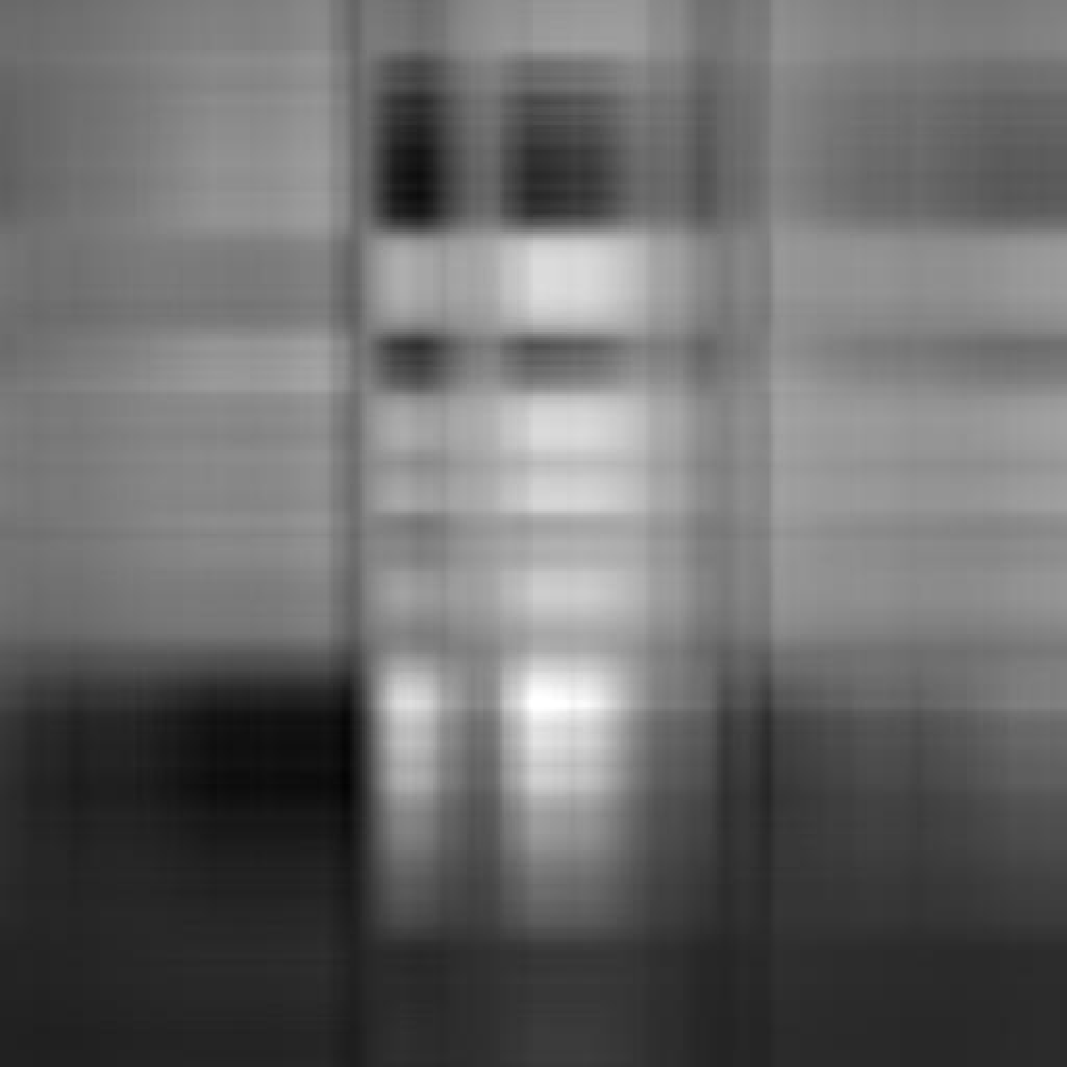
\includegraphics[width=0.3\columnwidth]{solution7.4_img/Alan_Turing_k=2.pdf}
                              & 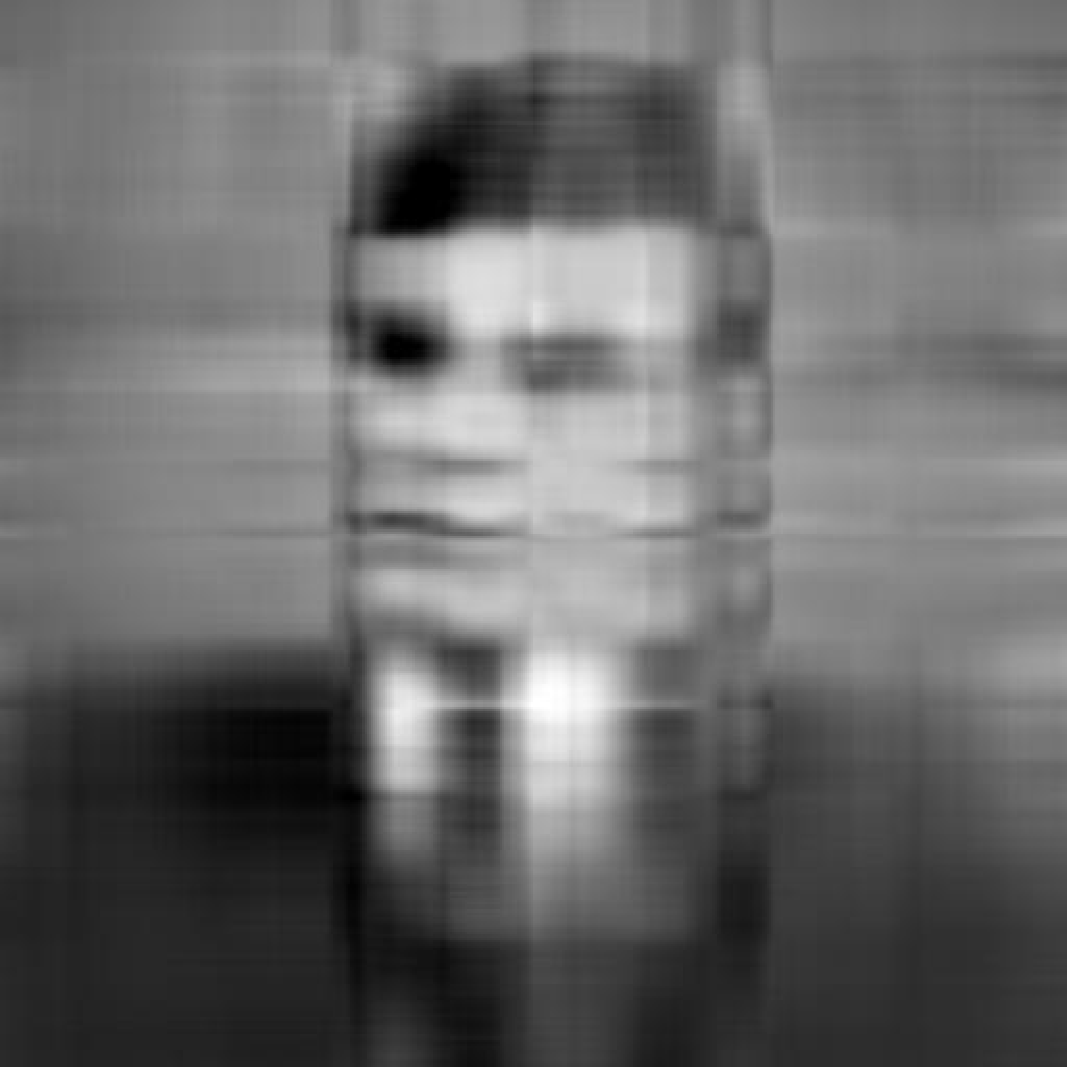
\includegraphics[width=0.3\columnwidth]{solution7.4_img/Alan_Turing_k=4.pdf}   \\
                      $k=2$   & $k=4$                                                                          \\
                      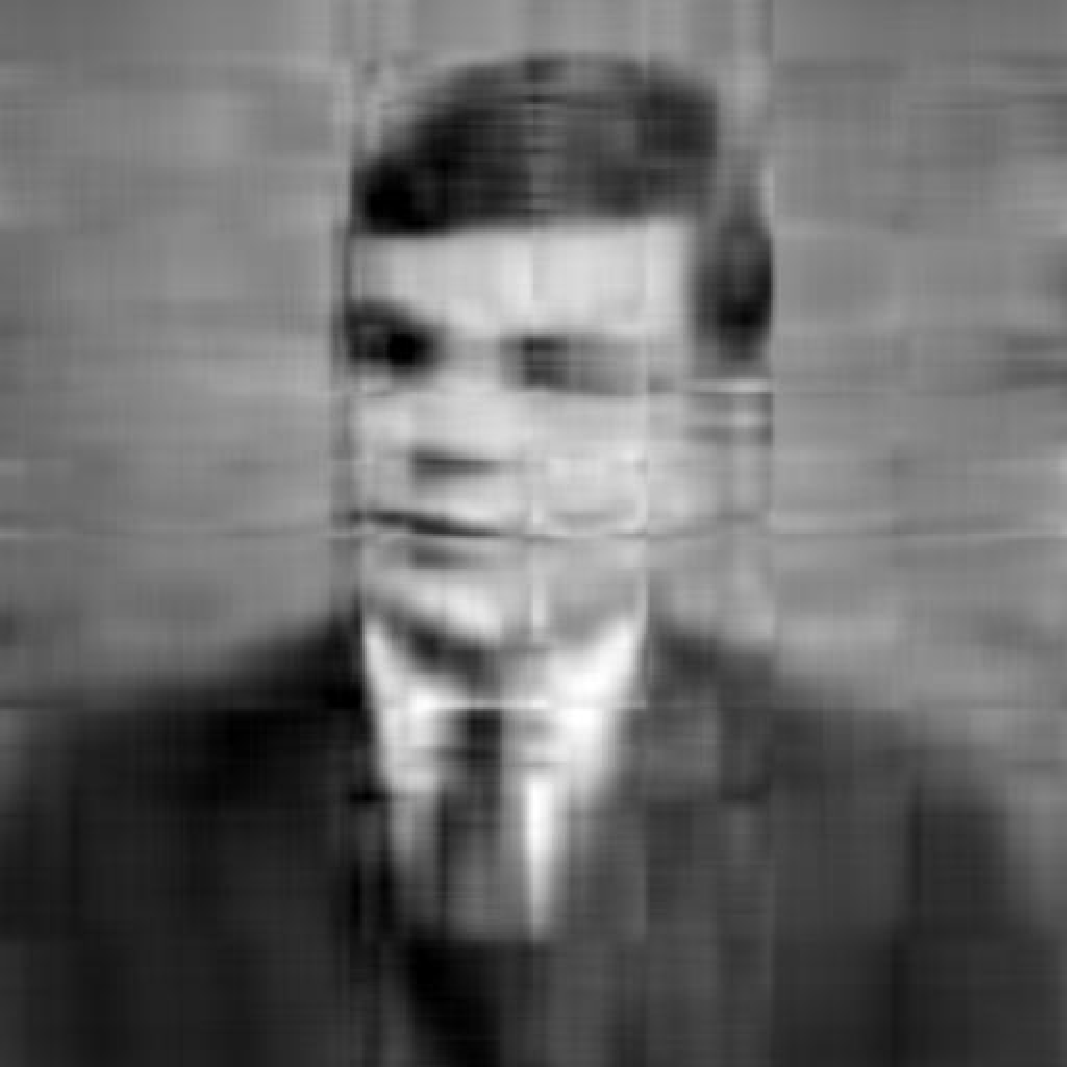
\includegraphics[width=0.3\columnwidth]{solution7.4_img/Alan_Turing_k=8.pdf}
                              & 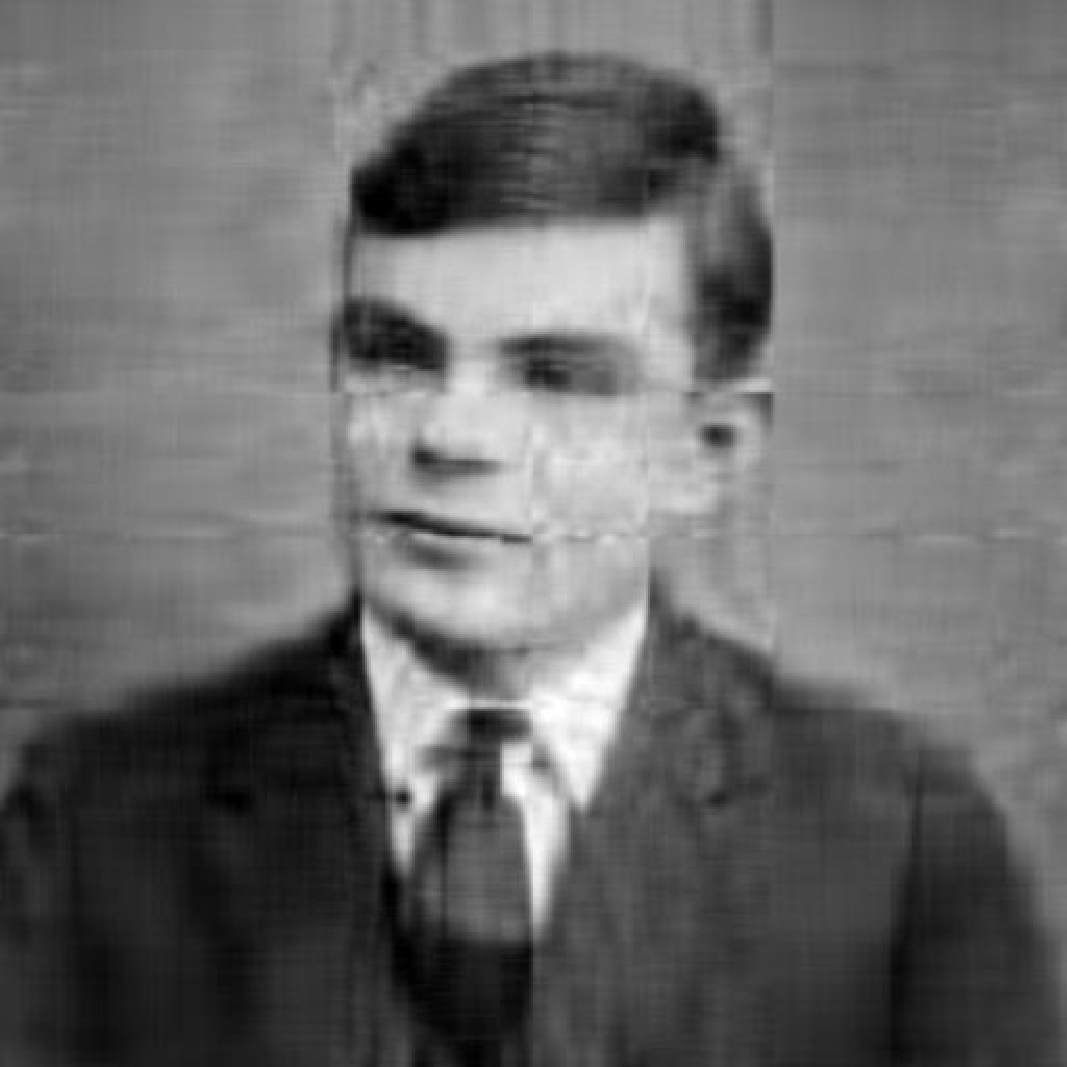
\includegraphics[width=0.3\columnwidth]{solution7.4_img/Alan_Turing_k=16.pdf}  \\
                      $k=8$   & $k=16$                                                                         \\
                      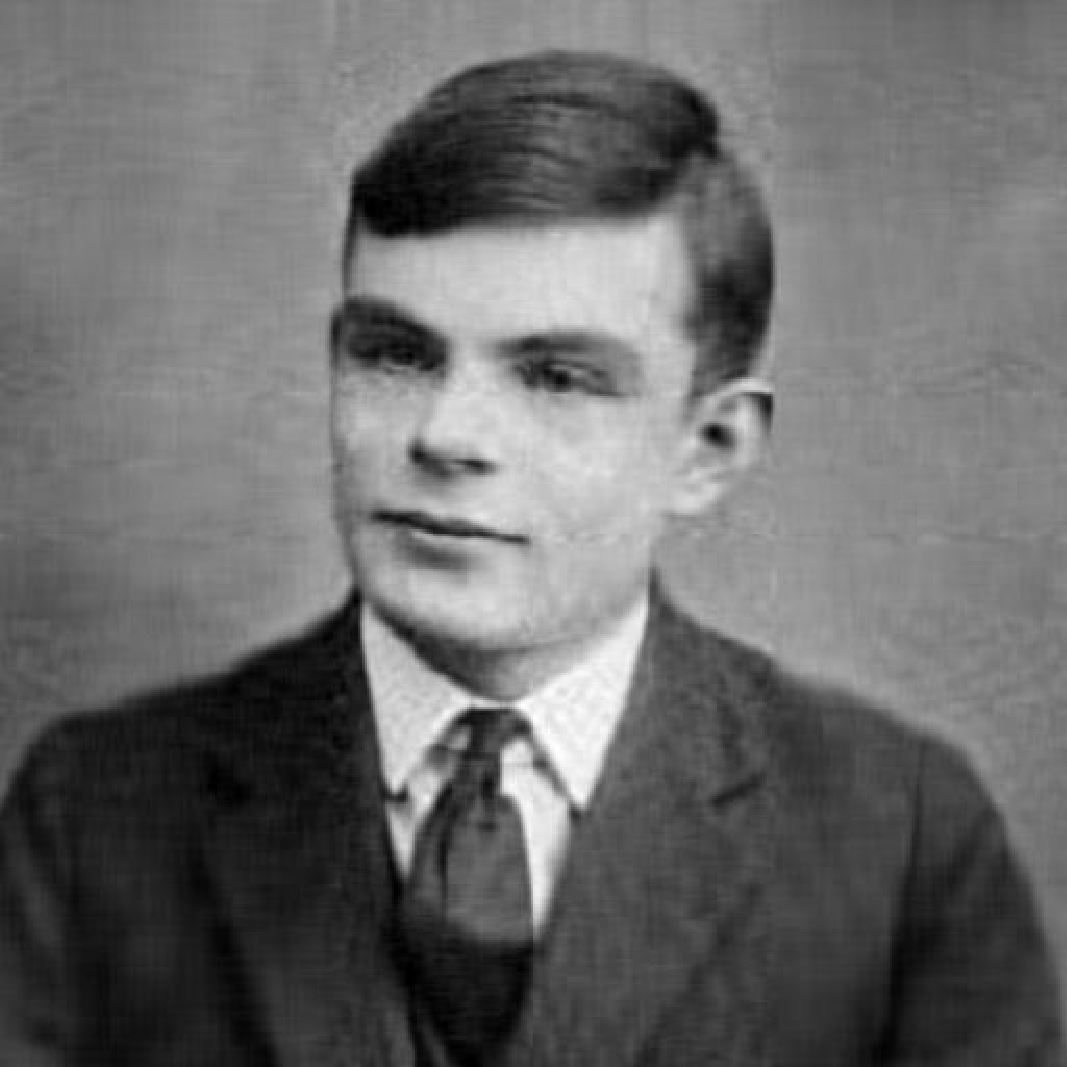
\includegraphics[width=0.3\columnwidth]{solution7.4_img/Alan_Turing_k=32.pdf}
                              & 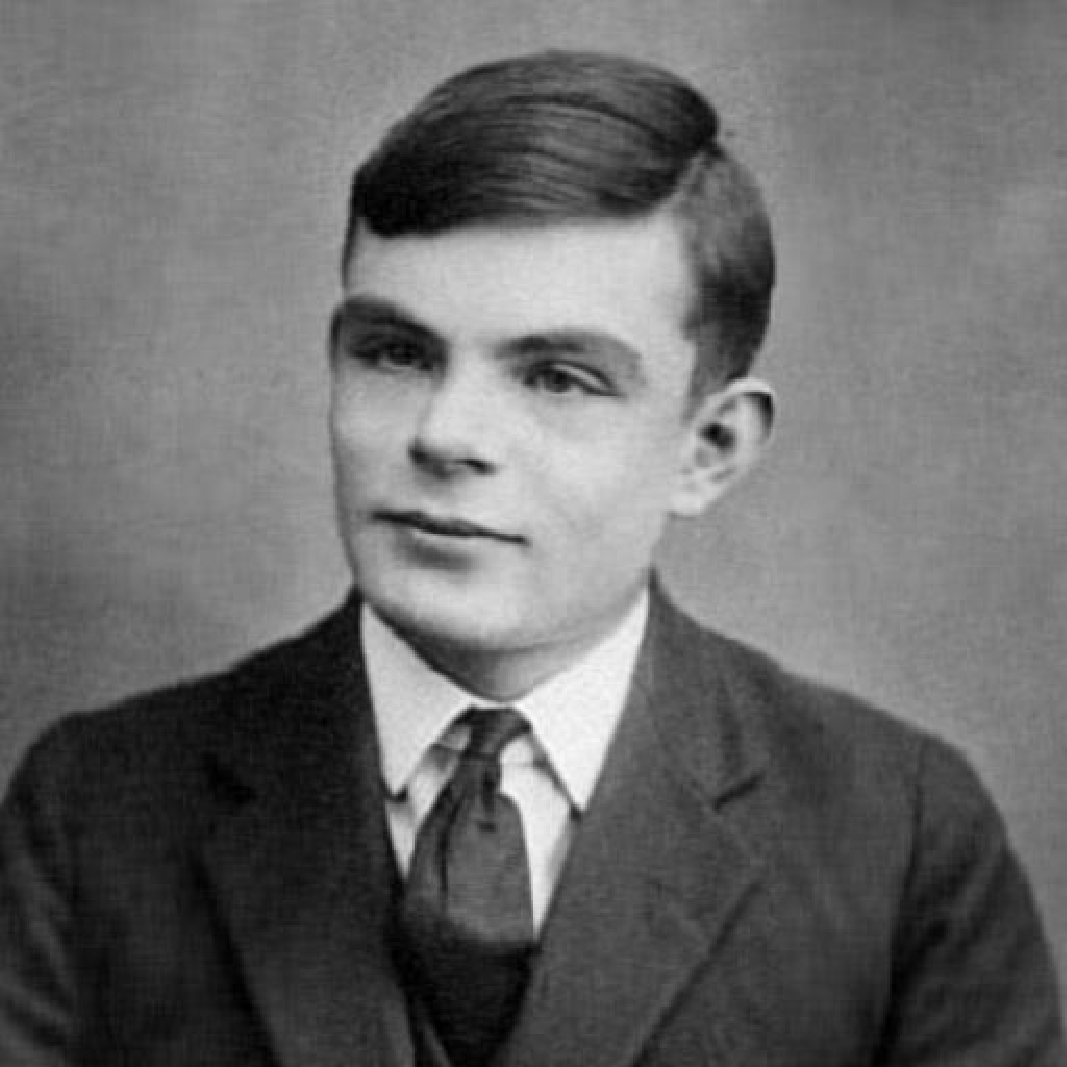
\includegraphics[width=0.3\columnwidth]{solution7.4_img/Alan_Turing_k=64.pdf}  \\
                      $k=32$  & $k=64$                                                                         \\
                      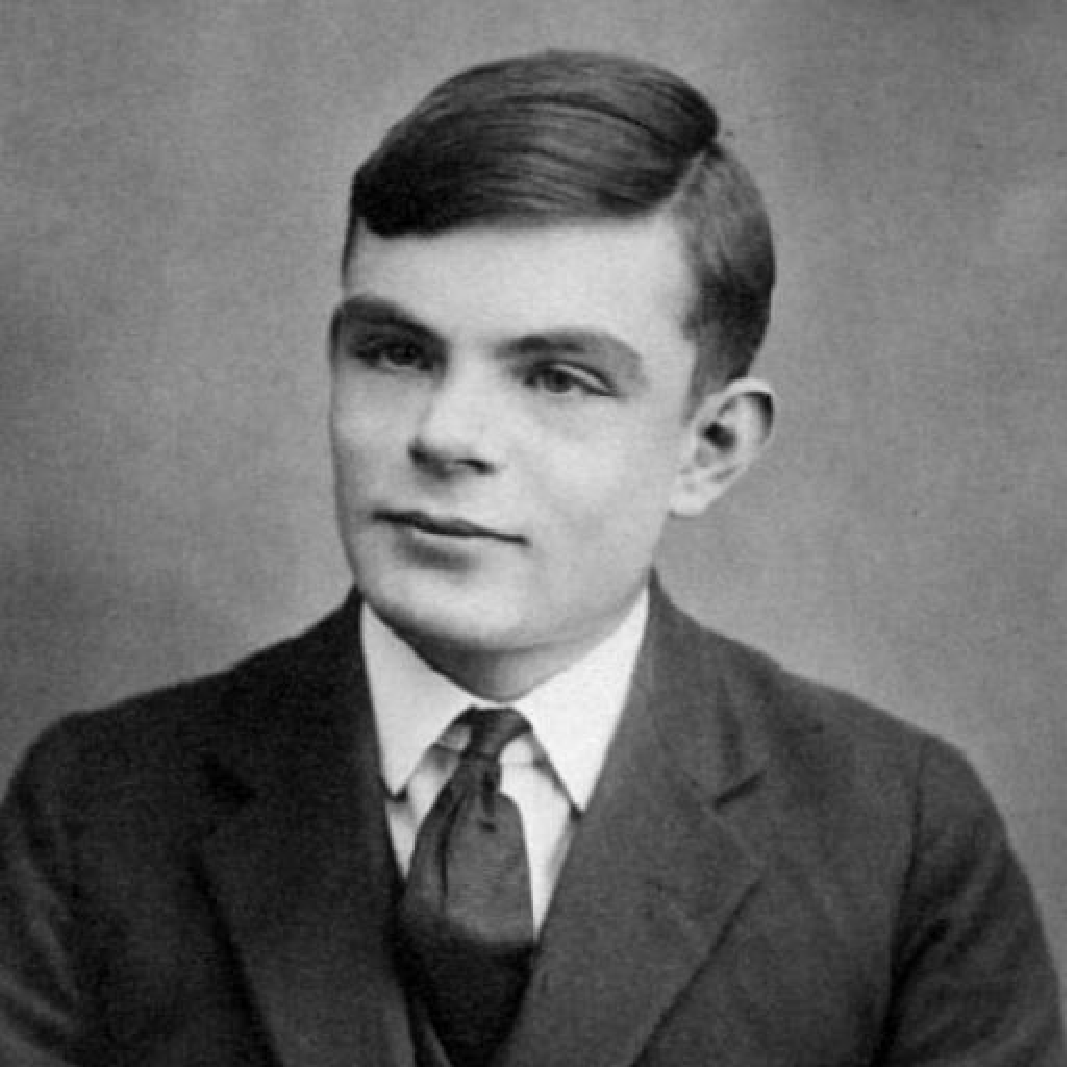
\includegraphics[width=0.3\columnwidth]{solution7.4_img/Alan_Turing_k=128.pdf}
                              & 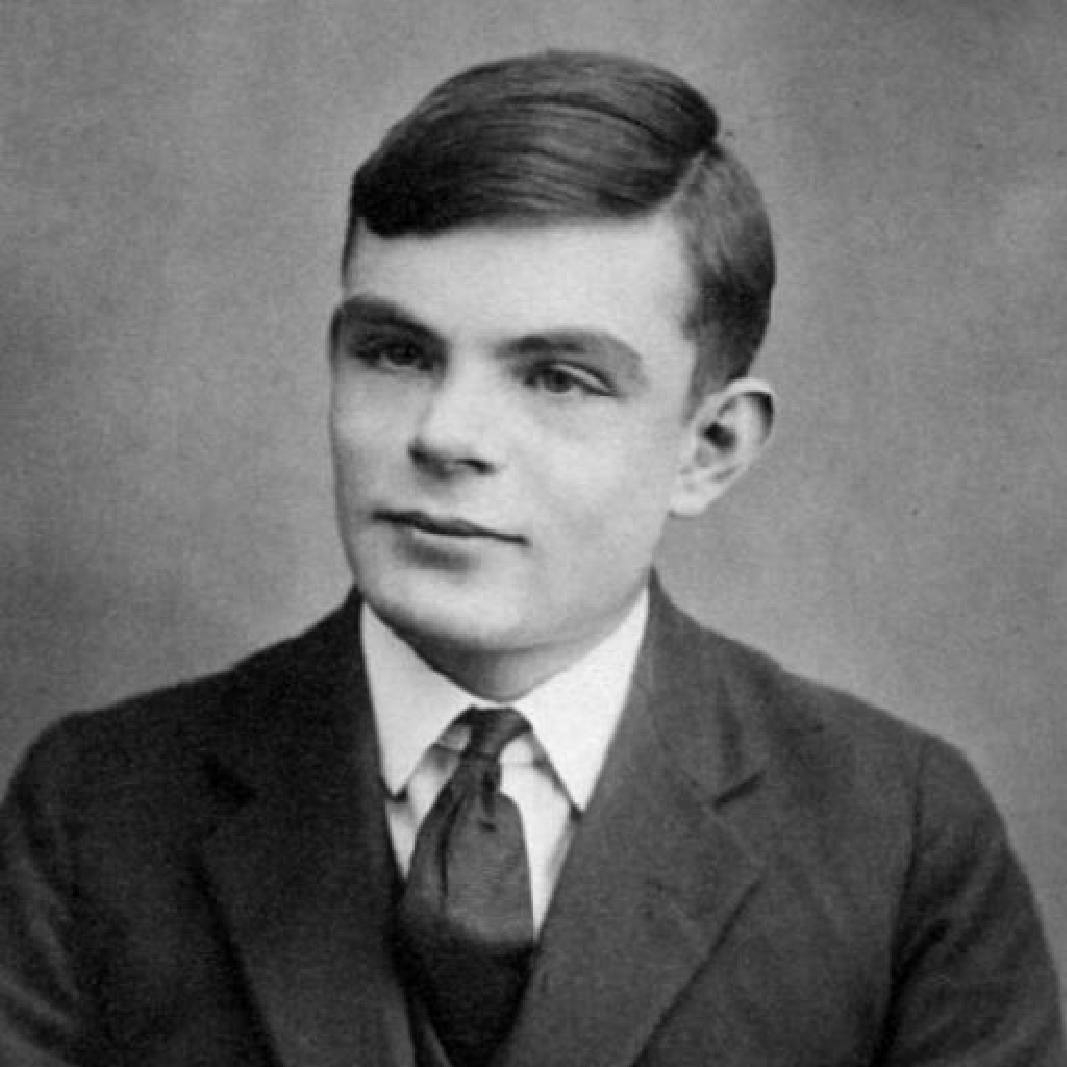
\includegraphics[width=0.3\columnwidth]{solution7.4_img/Alan_Turing_k=256.pdf} \\
                      $k=128$ & $k=256$
                  \end{tabular}
              \end{center}
    \end{enumerate}
\end{solution}

\newpage

\begin{exercise}[PCA \textnormal{60pts}]
    Suppose that we have a set of data instances $\{\mathbf{x}_i\}_{i=1}^n\subset\mathbb{R}^d$. Let $\widetilde{X}\in\mathbb{R}^{d\times n}$ be the matrix whose $i^{th}$ column is $\mathbf{x}_i-\Bar{\mathbf{x}}$, where $\Bar{\mathbf{x}}$ is the sample mean, and $S$ be the sample variance matrix.

    \begin{enumerate}
        \item For $G\in\mathbb{R}^{d\times K}$, let us define
              \begin{align}\label{eqn:obj-PCA}
                  f(G) = \tr(G^{\top}SG).
              \end{align}
              Show that $f(GQ)=f(G)$ for any orthogonal matrix $Q\in\mathbb{R}^{K\times K}$.

        \item Please find $\mathbf{g}_1$ defined as follows by the Lagrange multiplier method.
              \begin{align}\label{eqn:PC1}
                  \mathbf{g}_1:=\argmax_{\mathbf{g}\in\mathbb{R}^d}\{f(\mathbf{g}):\|\mathbf{g}\|_2=1\},
              \end{align}
              where $f$ is defined by (\ref{eqn:obj-PCA}). Notice that, the vector $\mathbf{g}_1$ is the first principle component vector of the data.

        \item Please find $\mathbf{g}_2$ defined as follows by the Lagrange multiplier method.
              \begin{align*}
                  \mathbf{g}_2:=\argmax_{\mathbf{g}\in\mathbb{R}^d}\{f(\mathbf{g}):\|\mathbf{g}\|_2=1,\langle\mathbf{g},\mathbf{g}_1\rangle=0\},
              \end{align*}
              where $\mathbf{g}_1$ is given by (\ref{eqn:PC1}). Similar to $\mathbf{g}_1$, the vector $\mathbf{g}_2$ is the second principle component vector of the data.

        \item Please derive the first $K$ principle component vectors by repeating the above process.

        \item What is $f(\mathbf{g}_k)$, $k=1,\ldots,K$? What about their meaning?

        \item When the first $K$ principle component vectors are unique?
    \end{enumerate}

\end{exercise}

\begin{solution}
    \begin{enumerate}
        \item  设 $Q=(\mathbf{q}_1,\cdots, \mathbf{q}_K)$
        $$\begin{aligned}
            f(GQ)
            &= \tr \left(Q^\top \left(G^\top S G\right) Q\right) \\
            &= \tr \left( \sum_{i=1}^K \sum_{j=1}^{K} \left(G^\top S G\right)_{i,j} \mathbf{q}_{i,*}^\top \mathbf{q}_{j,*} \right) \\
            &= \tr \left( \sum_{i=1}^{K} \left(G^\top S G\right)_{i,i} \right) \\
            &=\sum_{i=1}^{K} \left(G^\top S G\right)_{i,i} \\
            &=f(G)
        \end{aligned}$$
        \item $$f(\mathbf{g})
            =\tr \left( \mathbf{g}^\top S \mathbf{g}\right)
            =\mathbf{g}^\top S \mathbf{g}$$
            $$L(\lambda,\mathbf{g})=\mathbf{g}^\top S \mathbf{g}
            +\lambda(\mathbf{g}^\top \mathbf{g}-1)$$
            $$\nabla_\mathbf{g} L(\lambda,\mathbf{g})
            =\left( S^\top +S \right) \mathbf{g}+2\lambda \mathbf{g}
            =2S \mathbf{g}+2\lambda \mathbf{g}=0$$
            得到
            $$S\mathbf{g}=-\lambda \mathbf{g}$$ 
            所以 $$f(\mathbf{g})=-\lambda \mathbf{g}^\top \mathbf{g}=-\lambda$$
            而 $-\lambda$ 是 $S$ 的一个特征值,$f(\mathbf{g})$ 取最大值要求 $\lambda$ 取最大的特征值。\\
            所以 $\mathbf{g}_1$ 是 $S$ 的最大特征值对应的特征向量。
        \item $$L(\lambda,\mu,\mathbf{g})=\mathbf{g}^\top S \mathbf{g}+\lambda (\mathbf{g}^\top \mathbf{g})+\mu \mathbf{g}_1^\top \mathbf{g}$$
        $$\nabla_\mathbf{g} L(\lambda,\mu,\mathbf{g})
        =2S\mathbf{g}+2\lambda \mathbf{g}+\mathbf{g}_1=0$$
        所以 $$f(\mathbf{g})=\mathbf{g}^\top S\mathbf{g}=-\lambda$$
        同样的,$-\lambda$ 也是 $S$ 的特征值
        $\mathbf{g}_2$ 为 $S$ 的第二大的特征值对应的特征向量。
        \item 由上面两小题的规律可得,$\mathbf{g}_i$ 是 $S$ 的第 $i$ 大特征值对应的特征向量。
        \item $f(\mathbf{g}_k)$, 是 $S$ 的第 $k$ 大的特征值。
        \item 由上面小题易得,当前 $K$ 大的特征值都不相等时,前 $k$ 个 pronciple component 互不相等。
    \end{enumerate}
\end{solution}





%%%%%%%%%%%%%%%%%%%%%%%%%%%%%%%%%%%%%%%%%%%%%%%%%%%%%%%%%%%%%%%%

\end{document}
